\documentclass{beamer}
\usetheme{metropolis}

\usepackage[spanish]{babel}
\usepackage[utf8]{inputenc}
\usepackage{tikz}
\usepackage{xcolor}
\usepackage{amsmath}
\usepackage{listings}

% Definición de colores personalizados
\definecolor{primary}{RGB}{46, 204, 113}
\definecolor{secondary}{RGB}{52, 152, 219}
\definecolor{accent}{RGB}{231, 76, 60}
\definecolor{background}{RGB}{236, 240, 241}
\definecolor{gradient1}{RGB}{255, 107, 107}
\definecolor{gradient2}{RGB}{255, 159, 67}

% Configuración del tema
\setbeamercolor{normal text}{fg=black,bg=background}
\setbeamercolor{structure}{fg=primary}
\setbeamercolor{alerted text}{fg=accent}

\definecolor{lightgray}{rgb}{0.95,0.95,0.95}
\definecolor{darkgreen}{rgb}{0,0.5,0}
\definecolor{darkblue}{rgb}{0,0,0.5}

\lstset{
  backgroundcolor=\color{lightgray},
  basicstyle=\tiny\ttfamily,
  keywordstyle=\color{darkblue}\bfseries,
  commentstyle=\color{darkgreen},
  stringstyle=\color{red},
  numbers=left,
  numberstyle=\tiny\color{gray},
  stepnumber=1,
  numbersep=5pt,
  showspaces=false,
  showstringspaces=false,
  showtabs=false,
  frame=single,
  tabsize=2,
  language=Python,
  breaklines=true,
  breakatwhitespace=true
}

\title{\Huge\textbf{Python para I.O.}}
\author{Investigación Operativa, Universidad de San Andrés}
\date{}

\begin{document}

\begin{frame}
  \titlepage
\end{frame}

\begin{frame}{Motivación}
Python es un lenguaje de programación bastante versátil que nos va a permitir resolver problemas de optimización. Los pasos típicos van a ser:

\begin{enumerate}
    \item Identificar el problema
    \item Crear el modelo matemático
    \item Implementar y resolver usando Python
\end{enumerate}

\vspace{0.3cm}
En Investigación Operativa usamos Python porque los problemas con los que nos vamos a encontrar no son resolubles a mano.
\end{frame}

\begin{frame}{Proceso}
    \begin{tabular}{ccc}
    \textbf{Problema} & \hspace{0.5cm} $\rightarrow$ \hspace{0.5cm} \textbf{Modelado} \hspace{0.5cm} $\rightarrow$ \hspace{0.5cm} & \textbf{Optimización}
    \end{tabular}

    \begin{figure}[H]
        \centering
        \begin{tikzpicture}[node distance=2cm, auto, thick, scale=1.3, every node/.style={transform shape}]
            % Problema (izquierda)
            \foreach \i in {1,2,3} {
                \draw[fill=red!30] (-3,1.2-\i*0.8) circle (0.35) node {\i};
            }
            \foreach \i in {1,2,3,4} {
                \draw[fill=blue!20] (-2,1.5-\i*0.7) circle (0.32) node {\i};
            }
            % Conexiones
            \draw[thick, gray!70] (-3,0.4) -- (-2,0.8);
            \draw[thick, gray!70] (-3,0.4) -- (-2,0.1);
            \draw[thick, gray!70] (-3,0.4) -- (-2,-0.6);
            \draw[thick, gray!70] (-3,0.4) -- (-2,-1.3);
            \draw[thick, gray!70] (-3,-0.4) -- (-2,0.8);
            \draw[thick, gray!70] (-3,-0.4) -- (-2,0.1);
            \draw[thick, gray!70] (-3,-0.4) -- (-2,-0.6);
            \draw[thick, gray!70] (-3,-0.4) -- (-2,-1.3);
            \draw[thick, gray!70] (-3,-1.2) -- (-2,0.8);
            \draw[thick, gray!70] (-3,-1.2) -- (-2,0.1);
            \draw[thick, gray!70] (-3,-1.2) -- (-2,-0.6);
            \draw[thick, gray!70] (-3,-1.2) -- (-2,-1.3);
        \end{tikzpicture}
        \hfill
        \begin{tikzpicture}[node distance=2cm, auto, thick, scale=0.9, every node/.style={transform shape}]
            % Modelado (centro)
            \node[align=center] at (1.7,-0.2) {
                $Z = 3000x_1 + 5000x_2$\\[0.2em]
                $\begin{aligned}
                2x_2 &\leq 12\\
                3x_1 + 2x_2 &\leq 18\\
                x_1 &\geq 0 \\
                x_2 &\geq 0
                \end{aligned}$
            };
        \end{tikzpicture}
        \hfill
        \begin{tikzpicture}[node distance=2cm, auto, thick, scale=0.9, every node/.style={transform shape}]
            % Optimización (derecha)
            % Incluir imagen 3D
            \node[inner sep=0pt] at (5.5,1.2) {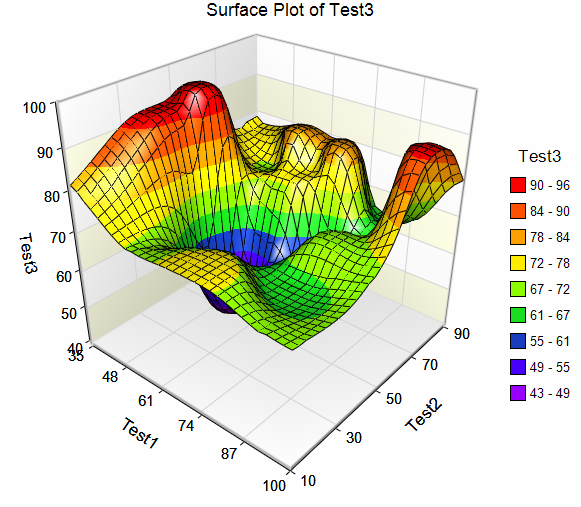
\includegraphics[width=4.2cm]{3d_graph.png}};
        \end{tikzpicture}
    \end{figure}
\end{frame}

\begin{frame}[fragile]{Variables en Python}
\begin{lstlisting}[numbers=left, numbersep=5pt]
texto = "Hello World"
numero = 5
numero_con_coma = 1.3
mi_lista = [1,2,3,4]
mi_tupla = (1,2,4)
\end{lstlisting}
\end{frame}

\begin{frame}{Operaciones}  
En Python podemos usar las operaciones matemáticas comunes escritas de la siguiente manera:

\begin{itemize}
    \item Suma: +
    \item Resta: \-
    \item Multiplicación: *
    \item División: /
    \item División entera: //
    \item Potencia: **
    \item Resto: \%
\end{itemize}
\end{frame}

\begin{frame}[fragile]{Print}
Si queremos imprimir una variable o el resultado de una operación usamos print:
\begin{lstlisting}[numbers=left, numbersep=5pt]
a = 10
b = 20
print("El resultado es", a+b)
# Output:
# El resultado es 30
\end{lstlisting}
\end{frame}

\begin{frame}{Listas}
Dada una lista a = [1,2,3] podemos realizar varias cosas:

\begin{itemize}
    \item Los elementos de a se pueden obtener haciendo a[i] donde i es la posición del elemento.
    \item ¡Ojo! En python el primer elemento es 0, no 1
    \item Podemos cambiar el elemento i de la lista escribiendo a[i] = 4
    \item Podemos agregar un elemento al final haciendo a.append(4)
\end{itemize}
\alert{(!) ¿Es lo mismo una lista y una tupla? ¿En qué difieren?}
\end{frame}

\begin{frame}[fragile]{Booleanos y Operadores Lógicos}
Los valores booleanos son True y False, y cuando comparamos dos variables, se nos devuelve el valor booleano correspondiente a esa relación.
\begin{itemize}
    \item \textbf{and}: Retorna True si AMBAS condiciones son True
    \item \textbf{or}: Retorna True si AL MENOS UNA condición es True
    \item \textbf{not}: Invierte el valor booleano
\end{itemize}
    
Ejemplo:
\begin{lstlisting}
a = True
b = False
print(a and b)  # False
print(a or b)   # True
print(not a)    # False
\end{lstlisting}
\end{frame}

\begin{frame}[fragile]{Operadores de Comparación}
Operadores lógicos:
\begin{itemize}
    \item $>$ Mayor que
    \item $<$ Menor que
    \item $==$ Igual (son dos porque si fuera uno sería asignación!)
    \item $\geq$ Mayor o igual
    \item $\leq$ Menor o igual
    \item $!=$ Distinto
\end{itemize}
\end{frame}

\begin{frame}[fragile]{If/else}
La sintaxis de if/else es la siguiente:

\begin{lstlisting}[numbers=left, numbersep=5pt]
if boolean:
    Statement1
else:
    Statement2

# Ejemplo:
if a == b:
    print(`Son iguales')
else:
    print(`Son distintos')
\end{lstlisting}

También es posible anidarlos o poner muchos condicionales con elif.
\end{frame}

\begin{frame}[fragile]{For loop}
La sintaxis del for loop que típicamente usaremos es la siguiente:

\begin{lstlisting}
for i in range(N):
    routine

# Ejemplo:
for i in range(4):
    print(i)

# Output:
# 0
# 1
# 2
# 3
\end{lstlisting}

La función range(N) genera una lista con una secuencia de números, hasta N-1.\\
Sintaxis: range(comienzo, final, paso)
\end{frame}

\begin{frame}[fragile]{While}
La sintaxis de while es la siguiente:

\begin{lstlisting}
while boolean:
    statement

# Ejemplo:
i = 0
while i < 4:
    print(i)
    i = i + 1
# Output:
# 0
# 1
# 2
# 3
\end{lstlisting}

¡Cuidado con los loops infinitos!
\end{frame}

\begin{frame}[fragile]{Librerías}
Vamos a usar en principio 4 librerías distintas:

\begin{itemize}
    \item \textbf{Numpy}: Para fácil manipulación de matrices y vectores
    \item \textbf{Matplotlib}: Nos va a permitir graficar funciones
    \item \textbf{PICOS}: Contiene paquetes de optimización que nos serán muy útiles
    \item \textbf{SciPy}: Para optimización no lineal
\end{itemize}

Este será nuestro estándar:
\begin{lstlisting}
import numpy as np
import scipy as scp
import picos
import matplotlib.pyplot as plt
\end{lstlisting}
\end{frame}

\begin{frame}[fragile]{Numpy}
Numpy nos permite trabajar con vectores y matrices fácilmente. El elemento básico que uno usa en Numpy son los `numpy arrays'

Para definir un Numpy array debemos escribirlo de la siguiente manera:

\begin{lstlisting}[numbers=left, numbersep=5pt]
array = np.array([1, 2, 3, 4])
\end{lstlisting}

Podemos acceder a los lugares del array de la misma forma que con las listas. La diferencia es que si en este caso tenemos una matriz y queremos ver el lugar i,j de la matriz podemos escribir array[i,j] en vez de array[i][j]

Además, en este caso, multiplicar un np.array por un escalar, equivale a multiplicar cada lugar del array por el escalar.
\end{frame}

\begin{frame}{Ejercicios Prácticos}
\textbf{Ejercicio 1: Listas y Promedios}
\begin{enumerate}
    \item Generar una lista L con todos los números pares hasta el 20
    \item Solo guardar los múltiplos de 4
    \item Calcular la media: $\langle L \rangle = \frac{\sum L_i}{N}$
\end{enumerate}

\textbf{Ejercicio 2: Función Múltiplos}
\begin{enumerate}
    \item Definir la función múltiplos que acepte como input el número hasta donde quiero obtener los números pares y el número del que quiero que sean múltiplos
    \item Graficar los puntos usando matplotlib
\end{enumerate}
\end{frame}

\begin{frame}{En fin...}
\begin{center}
\Huge\textbf{A programar se aprende programando}
\end{center}
\end{frame}

\end{document}